\documentclass[11pt]{article}

\usepackage[margin=1in]{geometry}
\usepackage{booktabs}
\usepackage{graphicx}
\usepackage{amsmath}
\usepackage{amssymb}
\usepackage{hyperref}

\hypersetup{colorlinks=true, linkcolor=blue, urlcolor=blue}

\newcommand{\sep}{\texttt{x}}
\newcommand{\subj}[1]{\texttt{a\_#1}}
\newcommand{\obj}[1]{\texttt{b\_#1}}
\newcommand{\rel}[1]{\texttt{r\_#1}}
\newcommand{\fatt}[1]{\texttt{f\_#1}}
\newcommand{\gatt}[1]{\texttt{g\_#1}}
\newcommand{\Rsem}{R_{\mathrm{sem}}}
\newcommand{\Rrnd}{R_{\mathrm{rnd}}}

\title{Linear and Nonlinear Relation Learning at Matched Frequency\\
\large Combined Goal 1 and Goal 2 Write-Up}
\author{factual-recall-mechanisms}
\date{2026-07-13}

\begin{document}
\maketitle

\section{Overview}

This document combines two claims tested in the same synthetic experiment. Goal~1
asks whether an infrequent, semantically supported relation can be learned in a
linear format. Goal~2 asks whether a frequent relation can be fully learned while
remaining nonlinear. A one-layer transformer is trained for exactly one epoch on
two relations with identical frequency statistics: a semantic relation $\Rsem$
supported by latent attributes and a balanced random relation $\Rrnd$ without such
support.

At $F{=}16$ occurrences per triple, $\Rsem$ is already learned and generalizes:
trained recall is $.672$, held-out recall is $.635$, and an affine probe reaches
$0.990 \pm 0.007$ accuracy. The frequency-matched random relation is barely learned
and its affine probe remains at chance. This is the Goal~1 infrequent/linear result.
At $F{=}64$, both relations reach perfect recall on all trained triples, but the
held-out affine probe is $0.891 \pm 0.056$ for $\Rsem$ and $0.016 \pm 0.022$ for
$\Rrnd$. This is the Goal~2 frequent/nonlinear result.

\section{Shared experimental setup}

\subsection{Data}

\paragraph{Vocabulary (265 tokens).}
A separator \sep; two relation tokens \rel{0}, \rel{1}; 192 subject tokens
$\subj{0},\dots,\subj{191}$; 32 object tokens $\obj{0},\dots,\obj{31}$; 32
attribute tokens $\fatt{0},\dots,\fatt{31}$; and 6 attribute tokens
$\gatt{0},\dots,\gatt{5}$.

\paragraph{Entities and attributes.}
Subject $\subj{i}$ carries
$(f_{i \bmod 32},g_{\lfloor i/32\rfloor})$. The 192 subjects therefore realize
each of the $32 \times 6$ attribute combinations exactly once. Object $\obj{j}$
carries $(f_{(j+3) \bmod 32},g_0)$.

\paragraph{Sentences.}
All training sentences have five tokens:
\begin{center}
\begin{tabular}{ll}
attribute sentence & \sep\ $\subj{i}$\ \fatt{p}\ \gatt{q}\ \sep
  \quad and \quad \sep\ $\obj{j}$\ \fatt{p}\ \gatt{q}\ \sep\\
relation triple & \sep\ $\subj{i}$\ $\rel{r}$\ $\obj{t}$\ \sep
\end{tabular}
\end{center}

\paragraph{Relations.}
\[
\Rsem(a_i)=b_{f(i)}, \qquad \Rrnd(a_i)=b_{\rho(i)},
\]
where $f(i)=i \bmod 32$ is the subject's own $f$-attribute index and $\rho$ is a
seed-dependent balanced random assignment onto the same 32 objects, independent of
the attributes. For seed 19, \subj{37} has attributes $(\fatt{5},\gatt{1})$, so
$\Rsem(\subj{37})=\obj{5}$ while $\Rrnd(\subj{37})=\obj{27}$.

\paragraph{Split and exact frequency matching.}
For every \fatt-value, 4 of its 6 subjects are trained and 2 are held out: 128
trained subjects and 64 held-out subjects. The random mapping is balanced within
both groups. Under both relations, every trained subject occurs in exactly one
triple, every object is the target of exactly 4 trained and 2 held-out subjects,
and both relations contribute 128 training triples repeated the same number of
times $F$. Held-out subjects appear in attribute sentences but never in relation
triples. These invariants are asserted by
\texttt{tests/test\_linear\_shift.py}.

\subsection{Model and training}

\begin{center}
\begin{tabular}{ll}
\toprule
Model & causal transformer, 1 layer, hidden 64, 4 heads, context 8\\
Embeddings & input and output embeddings untied; all weights
  $\mathcal{N}(0,0.02^2)$\\
 & no attribute-based initialization; nothing frozen; no loss reweighting\\
Parameters & 84{,}288\\
Corpus & every attribute sentence $\times A{=}128$ ($=28{,}672$ sentences)\\
 & $+$ 128 triples per relation, each $\times F$,
   $F\in\{1,4,16,64\}$\\
Training & exactly one epoch: one pass over the shuffled corpus\\
Steps & 452 ($F{=}1$) to 704 ($F{=}64$), batch size 64\\
Objective & unweighted next-token cross-entropy on all positions\\
Optimizer & AdamW, LR $10^{-3}$ after 5 warmup steps, weight decay 0,\\
 & gradient clip 1.0\\
Seeds & 19, 31, 47\\
\bottomrule
\end{tabular}
\end{center}

At $F{=}1$, every relation triple occurs exactly once in the model's complete
training history. At $F{=}64$, each triple occurs 64 times, but training is still a
single pass over one corpus.

\subsection{Metric and learning check}

The single analysis metric operationalizes the claim that a relation is an affine
transformation. Ordinary least-squares regression fits
\[
\hat o = \hat W s + \hat b
\]
from the subject input embedding $s_i\in\mathbb{R}^{64}$ to the target object's
unembedding row $o_{R(i)}\in\mathbb{R}^{64}$ using the 128 trained pairs. For each
of the 64 held-out subjects, the predicted vector is matched by cosine similarity
against all 32 object rows. Accuracy is the fraction for which the nearest row is
the unique correct object. Chance is $1/32\approx0.03$.

Greedy next-token recall on prompts \sep\ $\subj{i}$\ $\rel{r}$ is recorded as a
learning check. It distinguishes a relation whose representations admit an affine
map from a relation the model can actually recall.

\section{Goal 1: An infrequent relation is learned as linear}
\label{sec:goal1}

\subsection{Claim}

At low fact frequency, $F{=}16$ occurrences per triple in one epoch, $\Rsem$ is
genuinely learned: recall is $.672$ on trained triples and $.635$ on held-out
subjects never seen in a relation triple. What is learned is linear: the held-out
affine probe reaches $0.990\pm0.007$. The frequency-matched random control is barely
learned (trained recall $.167$) and its probe remains at chance.

\subsection{Results}

\begin{table}[htbp]
\centering
\begin{tabular}{rcccccc}
\toprule
 & \multicolumn{2}{c}{probe accuracy (held-out)}
 & \multicolumn{2}{c}{recall (trained)}
 & \multicolumn{2}{c}{recall (held-out)}\\
$F$ & $\Rsem$ & $\Rrnd$ & $\Rsem$ & $\Rrnd$ & $\Rsem$ & $\Rrnd$\\
\midrule
1 & $1.000\pm.000$ & $.031\pm.013$ & .029 & .010 & .016 & .010\\
4 & $1.000\pm.000$ & $.016\pm.013$ & .055 & .034 & .057 & .031\\
\textbf{16} & $\mathbf{0.990\pm.007}$ & $.036\pm.007$
  & \textbf{.672} & .167 & \textbf{.635} & .031\\
\midrule
control: no triples & $1.000\pm.000$ & $.021\pm.015$ & -- & -- & .000 & .000\\
\bottomrule
\end{tabular}
\caption{Goal~1 low-frequency cells, mean $\pm$ sd over seeds 19/31/47 at
$A{=}128$. The headline cell is $F{=}16$: $\Rsem$ is learned and linear, while
the frequency-matched $\Rrnd$ is barely learned and nonlinear.}
\label{tab:goal1}
\end{table}

\begin{figure}[htbp]
\centering
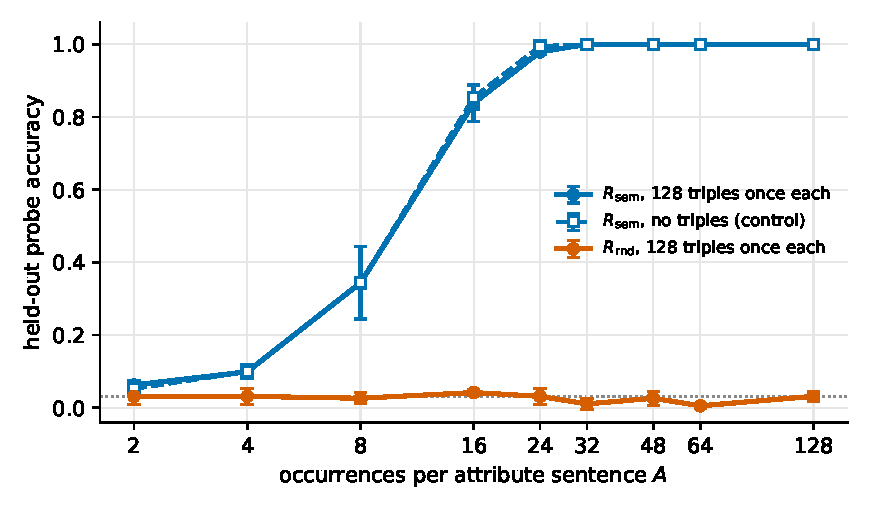
\includegraphics[width=0.72\textwidth]{figures/linear_shift_transition.pdf}
\caption{At $F{=}1$, probe accuracy as a function of attribute-sentence
occurrences $A$. The semantic transition from chance to ceiling is sharp and is
identical with 128 once-occurring triples (solid) and no triples (dashed control).
The random relation remains at chance.}
\label{fig:goal1-transition}
\end{figure}

\paragraph{Finding 1: at low frequency, what is learned is an affine map.}
With each fact occurring only 16 times, $\Rsem$ is learned on trained subjects,
generalizes to held-out subjects, and supports an almost perfect held-out affine
map. The frequency-matched random control is barely learned and remains at chance
under the probe. The semantic relation is learned earlier because it can use the
linear attribute structure.

\paragraph{Finding 2: the linear format is present at single occurrence.}
At $F{=}1$, the probe is already $1.000$ for $\Rsem$ and at chance for $\Rrnd$.
This is a representational statement: the model does not yet reproduce individual
triples behaviorally at $F{=}1$ (recall approximately $.03$).

\paragraph{Finding 3: the transition is driven by attribute knowledge.}
Sweeping $A$ at $F{=}1$ produces the probe sequence
$0.05\rightarrow0.10\rightarrow0.34\rightarrow0.85\rightarrow1.00$ for
$A=2,4,8,16,24$. The zero-triple control follows the same curve, showing that the
affine subject-to-object geometry is carried by attribute training rather than
triple repetition.

\subsection{Goal 1 scope}

The experiment shows an infrequent relation learned in a linear, generalizing
format and a sharp transition into the linear regime. It does not show that
single-occurrence relation triples cause that transition: the no-triple control
attributes it to scaffold exposure. Earlier single-exposure phase-shift results
using growing probe sets and attribute-initialized embeddings are superseded.

\section{Goal 2: A frequent relation is learned as nonlinear}
\label{sec:goal2}

\subsection{Claim}

At high fact frequency, $F{=}64$, both relations are fully learned: recall on all
128 trained triples is $1.000$ for both relations in all three seeds. Nevertheless,
the held-out affine probe reaches $0.891\pm0.056$ for $\Rsem$ and only
$0.016\pm0.022$ for $\Rrnd$, equal to chance. The frequent random relation is thus
stored without an affine map over the evaluated representations and does not
generalize to held-out subjects.

\subsection{Results}

\begin{table}[htbp]
\centering
\begin{tabular}{rcccccc}
\toprule
 & \multicolumn{2}{c}{probe accuracy (held-out)}
 & \multicolumn{2}{c}{recall (trained)}
 & \multicolumn{2}{c}{recall (held-out)}\\
$F$ & $\Rsem$ & $\Rrnd$ & $\Rsem$ & $\Rrnd$ & $\Rsem$ & $\Rrnd$\\
\midrule
1 & $1.000\pm.000$ & $.031\pm.013$ & .029 & .010 & .016 & .010\\
4 & $1.000\pm.000$ & $.016\pm.013$ & .055 & .034 & .057 & .031\\
16 & $0.990\pm.007$ & $.036\pm.007$ & .672 & .167 & .635 & .031\\
\textbf{64} & $0.891\pm.056$ & $\mathbf{.016\pm.022}$
  & \textbf{1.000} & \textbf{1.000} & .995 & \textbf{.031}\\
\bottomrule
\end{tabular}
\caption{Goal~2 frequency sweep, mean $\pm$ sd over seeds 19/31/47 at
$A{=}128$. At $F{=}64$, both relations are fully recalled on trained triples, but
only $\Rsem$ admits a held-out affine map.}
\label{tab:goal2}
\end{table}

\begin{figure}[htbp]
\centering
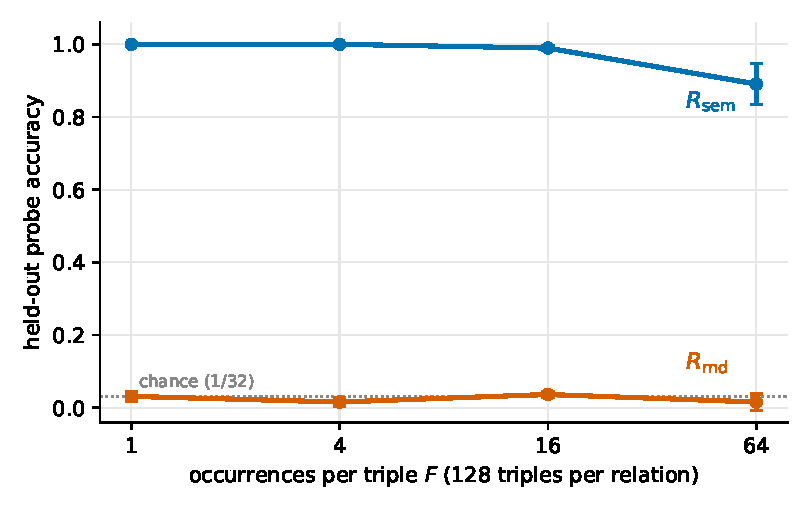
\includegraphics[width=0.65\textwidth]{figures/linear_shift_fsweep.pdf}
\caption{Held-out probe accuracy versus occurrences per triple for the two
frequency-matched relations. The random relation stays at chance while the
semantic relation remains high, with mild erosion at $F{=}64$.}
\label{fig:goal2-fsweep}
\end{figure}

\paragraph{Finding 1: a fully learned frequent relation without held-out affine structure.}
At 64 occurrences per triple, $\Rrnd$ reaches perfect recall of every trained
triple while its held-out probe and held-out behavioral recall remain at chance.
It is therefore a non-generalizing memorization under the stated affine metric.

\paragraph{Finding 2: the contrast is due to semantics, not frequency.}
The semantic relation is trained in the same model with exactly the same frequency,
is equally well recalled, and retains high affine-probe and held-out recall. Raising
$\Rrnd$ from 1 to 64 occurrences changes whether it is recalled but never lifts its
held-out affine score above chance.

\paragraph{Finding 3: high frequency mildly erodes semantic linearity.}
The $\Rsem$ probe declines from $1.000$ at $F\leq4$ to $0.891\pm0.056$ at
$F{=}64$, consistent with high-frequency memorization competing with the linear
solution while leaving it far above the random relation.

\subsection{Goal 2 scope}

The precise claim is not that frequency always causes nonlinearity. At matched high
frequency, the attribute-supported relation remains largely linear while the
unsupported random relation is fully recalled without held-out affine transfer.
Earlier high-frequency experiments using structured embedding initialization,
targeted-row updates, or top-$k$ metrics are superseded by this end-to-end setup.

\section{Joint conclusion}

The two goals establish complementary regimes in one frequency-controlled
experiment. Semantic structure permits an affine, generalizing solution before the
random control is well learned. With enough repetition, the random relation can be
perfectly recalled on its training facts without acquiring held-out affine transfer.
Frequency controls whether unsupported facts are memorized; semantic support
controls whether the learned relation aligns with a transferable affine geometry.

\section{Reproduction}

Implementation: \path{experiments/factual_recall/linear_shift.py}.

Design invariants: \path{experiments/tests/test_linear_shift.py}.

Run the following commands from \texttt{experiments/}:

\begin{small}
\begin{verbatim}
# Tables and Goal 2 frequency figure; run separately for seeds 19, 31, and 47
uv run python -m factual_recall.linear_shift --world category --probe embedding \
  --seeds 19 --k-values 0,128 --occurrences 1,4,16,64 --attr-repeats 128 \
  --device cuda --output-dir factual_recall/results/final_category_seed19

# Goal 1 transition figure; repeat for each seed and A in
# {2,4,8,16,24,32,48,64,128}
uv run python -m factual_recall.linear_shift --world category --probe embedding \
  --seeds 19 --k-values 0,128 --occurrences 1 --attr-repeats 8 \
  --device cuda \
  --output-dir factual_recall/results/final_category_arsweep_seed19_ar8

uv run pytest tests/test_linear_shift.py -q
\end{verbatim}
\end{small}

Raw metrics are in
\path{factual_recall/results/final_category_*/linear_shift_metrics.json}.
The source claims remain available separately in
\texttt{goal1\_infrequent\_relation\_linear.tex} and
\texttt{goal2\_frequent\_relation\_nonlinear.tex}.

\end{document}
